\documentclass[journal,10pt,twocolumn]{article}
\usepackage{graphicx, float}
\usepackage[margin=0.5in]{geometry}
\usepackage{amsmath, bm}
\usepackage{array}
\usepackage{booktabs}
\providecommand{\norm}[1]{\left\lVert#1\right\rVert}
\let\vec\mathbf
\newcommand{\myvec}[1]{\ensuremath{\begin{pmatrix}#1\end{pmatrix}}}
\newcommand{\mydet}[1]{\ensuremath{\begin{vmatrix}#1\end{vmatrix}}}

\title{\textbf{Circle Assignment}}
\author{A L U R U A J A Y}
\date{September 2022}

\begin{document}

\maketitle
\paragraph{\textit{Problem Statement} -A square is inscribed in the circle $x^2$+$y^2$-2x+4y+3=0.Whose sides are parallel to the coordinate axes,Find out the vertexes of the square.}

\section{CONSIDERATIONS}
\vspace{0.2cm}
The input parameters are the r, a and c. \\
\vspace{0.2cm}
{

\setlength\extrarowheight{2pt}
\begin{tabular}{|c|c|c|}
	\hline
	\textbf{Symbol}&\textbf{Value}&\textbf{Description}\\
	\hline
	r&r& radius of a circle\\
	\hline
	a&a&side of a square\\
	\hline
	c&c&centre of a circle\\
	\hline
\end{tabular}
}
\section{DIAGRAM}
Plot of square in a circle is shown in figure 1, where point O is Center and points A, B, C and D are the vertices of Square.
\begin{figure}[h]
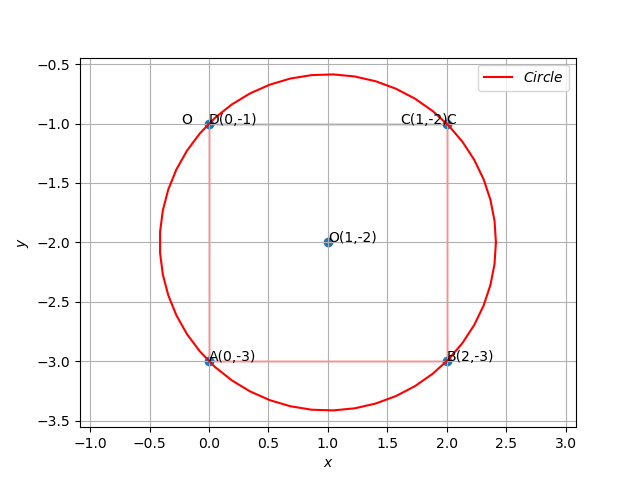
\includegraphics[scale=0.6]{circle.png}
\caption{Circle}
\label{fig:Circle}
\end{figure}

\section{Solution}

\vspace{0.25cm}
\subsection{Calculation of Centre and Radius of a Circle}
\begin{flushleft}
Equation of the circle is
\begin{equation}
x^2+y^2-2x+4y+3=0 
\end{equation}
\end{flushleft}
The equation of circle in matrix form is,
\begin{equation}
 \vec{x}^T \vec{V} \vec{x} + 2 \vec{u}^T \vec{x} + f = 0
\end{equation}
\begin{flushleft}
Where\\
\end{flushleft}
\begin{center}
\begin{math}
\vec{V} = \vec{I}= \myvec{ 1 & 0\\ 0 & 1} , \vec{u} = \myvec{-1 \\ 2}, f=3
\end{math}
\end{center}
\endcenter
\begin{flushleft}
We know that
\vspace{0.3cm}\\
radius (r)= \begin{math}
\sqrt{\vec{u}^T \vec{u} -f}\end{math}
\vspace{0.3cm}\\
centre(O)=$-\vec{u}$ 
\end{flushleft}
\begin{flushleft}
\subsection{Finding Co-Ordinate C}
let The parametric equation of a line is given by
\begin{equation}
  \boldsymbol{x}= \vec{e}+\lambda_1(\vec{m}_1)   
\end{equation}
Point on the $||\vec{B-C}||$ = 
\begin{math}
\vec{e} =
\end{math}
\begin{math}
1 \times \vec{e}_1 =
\end{math}
\begin{math}
\myvec{2 \\ -2}
\end{math}
\vspace{0.3cm}\\
Direction Vector of a line  $||\vec{B-C}||$ = 
\begin{math}
\vec{m}_1 = \myvec{0 \\ 1}
\end{math}
\vspace{0.3cm}\\
from eq(3) The parametric equation of a line can be written as
\begin{equation}
     \boldsymbol{x} = \myvec{-1 \\ 2} + \lambda_1\myvec{0 \\ 1}
\end{equation}
let The parametric equation of a line is given by
\begin{equation}
 \boldsymbol{x} = \vec{f}+\lambda_2(\vec{m}_2)   
\end{equation}
Point on the $||\vec{C-D}||$ = 
\begin{math}
\vec{f} =
\end{math}
\begin{math}
1 \times \vec{e}_2 =
\end{math}
\begin{math}
\myvec{0 \\ 1}
\end{math}
\vspace{0.3cm}\\
Direction Vector of a line  $||\vec{C-D}||$ = 
\begin{math}
\vec{m}_2 = \myvec{0 \\ 1}
\end{math}
\vspace{0.3cm}\\
from eq(5) The parametric equation of a line can be written as
\begin{equation}
     \boldsymbol{x} = \myvec{1 \\ -1} + \lambda_2\myvec{1 \\ 0}
\end{equation}
\vspace{0.3cm}\\
By solving eq(4) $\And$ eq(6),we get
\vspace{0.3cm}\\
 \myvec{\lambda_1 \\ \lambda_2} =  \myvec{1 \\ 1}
\vspace{0.3cm}\\
$\lambda_1=1 \And \lambda_2=1$
\vspace{0.3cm}\\
Sub the value of $\lambda_1$in eq(4),then we get the Co-ordinate of C
\vspace{0.3cm}\\
C =  \myvec{2 \\ -2} + 1  \myvec{0 \\ 1}
\vspace{0.3cm}\\
C = \myvec{2 \\ -1}
\subsection{Finding Co-Ordinate A}
let The parametric equation of a line is given by
\begin{equation}
 \boldsymbol{x} = \vec{g}+\lambda_3(\vec{m}_1)   
\end{equation}
Point on the $||\vec{A-D}||$ = 
\begin{math}
\vec{g} =
\end{math}
\begin{math}
1 \times \vec{e}_1 =
\end{math}
\begin{math}
\myvec{0 \\ -2}
\end{math}
\vspace{0.3cm}\\
Direction Vector of a line  $||\vec{A-D}||$ = 
\begin{math}
\vec{m}_1 = \myvec{0 \\ 1}
\end{math}
\vspace{0.3cm}\\
from eq(7) The parametric equation of a line can be written as
\begin{equation}
     \boldsymbol{x} = \myvec{0 \\ -2} + \lambda_3\myvec{0 \\ 1}
\end{equation}
let The parametric equation of a line is given by
\begin{equation}
 \boldsymbol{x} = \vec{h}+\lambda_4(\vec{m}_2)   
\end{equation}
Point on the $||\vec{C-D}||$ = 
\begin{math}
\vec{h} =
\end{math}
\begin{math}
1 \times \vec{e}_2 =
\end{math}
\begin{math}
\myvec{1 \\ -3}
\end{math}
\vspace{0.3cm}\\
Direction Vector of a line  $||\vec{C-D}||$ = 
\begin{math}
\vec{m}_2 = \myvec{1 \\ 0}
\end{math}
\vspace{0.3cm}\\
from eq(9) The parametric equation of a line can be written as
\begin{equation}
     \boldsymbol{x} = \myvec{1 \\ -3} + \lambda_4\myvec{1 \\ 0}
\end{equation}
By solving eq(8) $\And$ eq(10),we get
\vspace{0.3cm}\\
 \myvec{\lambda_3 \\ \lambda_4} =  \myvec{-1 \\ -1}
\vspace{0.3cm}\\
$\lambda_3=-1 \And \lambda_4=-1$
\vspace{0.3cm}\\
Sub the value of $\lambda_1$in eq(8),then we get the Co-ordinate of A
\vspace{0.3cm}\\
A =  \myvec{0 \\ -2} + -1  \myvec{0 \\ 1}
\vspace{0.3cm}\\
A = \myvec{0 \\ -3}
\subsection{Finding Co-Ordinate B}
Let The parametric equation of a line is given by
\begin{equation}
 \boldsymbol{x} = \vec{h}+\lambda_4(\vec{m}_2)   
\end{equation}
Point on the $||\vec{C-D}||$ = 
\begin{math}
\vec{h} =
\end{math}
\begin{math}
1 \times \vec{e}_2 =
\end{math}
\begin{math}
\myvec{1 \\ -3}
\end{math}
\vspace{0.3cm}\\
Direction Vector of a line  $||\vec{C-D}||$ = 
\begin{math}
\vec{m}_2 = \myvec{1 \\ 0}
\end{math}
\vspace{0.3cm}\\
from eq(11) The parametric equation of a line can be written as
\begin{equation}
     \boldsymbol{x} = \myvec{1 \\ -3} + \lambda_4\myvec{1 \\ 0}
\end{equation}
t The parametric equation of a line is given by
\begin{equation}
 \boldsymbol{x} = \vec{e}+\lambda_1(\vec{m}_1)   
\end{equation}
Point on the $||\vec{B-C}||$ = 
\begin{math}
\vec{e} =
\end{math}
\begin{math}
1 \times \vec{e}_1 =
\end{math}
\begin{math}
\myvec{2 \\ -2}
\end{math}
\vspace{0.3cm}\\
Direction Vector of a line  $||\vec{B-C}||$ = 
\begin{math}
\vec{m}_1 = \myvec{0 \\ 1}
\end{math}
\vspace{0.3cm}\\
from eq(13) The parametric equation of a line can be written as
\begin{equation}
     \boldsymbol{x} = \myvec{-1 \\ 2} + \lambda_1\myvec{0 \\ 1}
\end{equation}
By solving eq(12) $\And$ eq(14),we get
\vspace{0.3cm}\\
 \myvec{\lambda_4 \\ \lambda_1} =  \myvec{1 \\ -1}
\vspace{0.3cm}\\
$\lambda_4=1 \And \lambda_1=-1$
\vspace{0.3cm}\\
Sub the value of $\lambda_1$in eq(12),then we get the Co-ordinate of B
\vspace{0.3cm}\\
B =  \myvec{1 \\ -3} + 1  \myvec{1 \\ 0}
\vspace{0.3cm}\\
B = \myvec{2 \\ -3}
\subsection{Finding Co-Ordinate D}
let The parametric equation of a line is given by
\begin{equation}
 \boldsymbol{x} = \vec{g}+\lambda_3(\vec{m}_1)   
\end{equation}
Point on the $||\vec{A-D}||$ = 
\begin{math}
\vec{g} =
\end{math}
\begin{math}
1 \times \vec{e}_1 =
\end{math}
\begin{math}
\myvec{0 \\ -2}
\end{math}
\vspace{0.3cm}\\
Direction Vector of a line  $||\vec{A-D}||$ = 
\begin{math}
\vec{m}_1 = \myvec{0 \\ 1}
\end{math}
\vspace{0.3cm}\\
from eq(15) The parametric equation of a line can be written as
\begin{equation}
     \boldsymbol{x} = \myvec{0 \\ -2} + \lambda_3\myvec{0 \\ 1}
\end{equation}
let The parametric equation of a line is given by
\begin{equation}
 \boldsymbol{x} = \vec{f}+\lambda_2(\vec{m}_2)   
\end{equation}
Point on the $||\vec{C-D}||$ = 
\begin{math}
\vec{f} =
\end{math}
\begin{math}
1 \times \vec{e}_2 =
\end{math}
\begin{math}
\myvec{0 \\ 1}
\end{math}
\vspace{0.3cm}\\
Direction Vector of a line  $||\vec{C-D}||$ = 
\begin{math}
\vec{m}_2 = \myvec{0 \\ 1}
\end{math}
\vspace{0.3cm}\\
from eq(17) The parametric equation of a line can be written as
\begin{equation}
     \boldsymbol{x} = \myvec{1 \\ -1} + \lambda_2\myvec{1 \\ 0}
\end{equation}
\vspace{0.3cm}\\
By solving eq(4) $\And$ eq(6),we get
\vspace{0.3cm}\\
 \myvec{\lambda_2 \\ \lambda_3} =  \myvec{-1 \\ 1}
\vspace{0.3cm}\\
$\lambda_2=-1 \And \lambda_3=1$
\vspace{0.3cm}\\
Sub the value of $\lambda_1$in eq(4),then we get the Co-ordinate of C
\vspace{0.3cm}\\
D =  \myvec{0 \\ -2} + 1  \myvec{0 \\ 1}
\vspace{0.3cm}\\
D = \myvec{0 \\ -1}
\subsection{Conclusion}
The Vertexes of square are
\vspace{0.3cm}\\
A = \myvec{0 \\ -3} B = \myvec{2 \\ -3} C = \myvec{2 \\ -1} D = \myvec{0 \\ -1}
\end{flushleft}
\end{document}
